%%%%%%%%%%%%%%%%%%%%%%%%%%%%%%%%%%%%%%%%%
% Stylish Article
% LaTeX Template
% Version 1.0 (31/1/13)
%
% This template has been downloaded from:
% http://www.LaTeXTemplates.com
%
% Original author:
% Mathias Legrand (legrand.mathias@gmail.com)
%
% License:
% CC BY-NC-SA 3.0 (http://creativecommons.org/licenses/by-nc-sa/3.0/)
%
%%%%%%%%%%%%%%%%%%%%%%%%%%%%%%%%%%%%%%%%%

%----------------------------------------------------------------------------------------
%	PACKAGES AND OTHER DOCUMENT CONFIGURATIONS
%----------------------------------------------------------------------------------------

\documentclass[fleqn,10.5pt,ngerman]{SelfArx}

\usepackage{babel}
\selectlanguage{ngerman}

\setlength{\columnsep}{0.55cm} % Distance between the two columns of text
\setlength{\fboxrule}{0.75pt} % Width of the border around the abstract

\definecolor{color1}{RGB}{0,0,90} % Color of the article title and sections
\definecolor{color2}{RGB}{0,20,20} % Color of the boxes behind the abstract and headings

\newlength{\tocsep} 
\setlength\tocsep{1.5pc} % Sets the indentation of the sections in the table of contents
\setcounter{tocdepth}{2} % Show only three levels in the table of contents section: sections, subsections and subsubsections


\usepackage{fontenc}
\usepackage{inputenc}
\usepackage{url} 
\usepackage{listings}

%----------------------------------------------------------------------------------------
%	ARTICLE INFORMATION
%----------------------------------------------------------------------------------------

\JournalInfo{Bericht zur Praktische Studienphase} % Journal information
\Archive{Wintersemester 16/17} % Additional notes (e.g. copyright, DOI, review/research article)

\PaperTitle{REpresentational State Transfer - Architekturstil} % Article title

\Authors{Felix Scheidel} % Authors
\affiliation{\textit{Hochschule Kaiserslautern}} % Author affiliation
\affiliation{\textbf{Corresponding author}: fesc0013@stud.hs-kl.de} % Corresponding author

\Keywords{Web-Entwicklung, RESTful, SOA, JSON, WSA, SOAP, Java} % Keywords - if you don't want any simply remove all the text between the curly brackets
\newcommand{\keywordname}{Keywords} % Defines the keywords heading name

%----------------------------------------------------------------------------------------
%	ABSTRACT
%----------------------------------------------------------------------------------------
\Abstract{Im Zuge der praktischen Studienphase bei der Bosch Software Innovations GmbH wurden viele Erfahrungen mit Technololgien und praktischen Ansätzen gesammelt. Einer dieser Ansätze ist das Realisieren von Web-Applikationen unter Verwendung des REST-Architekturstils. Was ist REST und wo kommt es zum Einsatz? Behandelt werden in Folgendem die grundlegenden Eigenschaften die eine REST-Schnittstelle als solche auszeichnet und was REST von zum Beispiel SOAP unterscheidet. An einer Beispielimplementierung werden einige der Eigenschaften verdeutlicht und genauer beschrieben.}


%----------------------------------------------------------------------------------------

\begin{document}
%----------------- ABSTRACT -----------------%
%----------------- KONFIGURATION ----------------- %
\thispagestyle{empty}

\section*{Kurzfassung}
\label{cha:kurzfassung}
Im Zuge meiner praktischen Studienphase wurde ich bei der Bosch Software Innovations GmbH mit vielen Technologien, technischen Ansätzen und Konventionen in der modernen Softwareentwicklung konfrontiert. Durch diese Erfahrungen entstand der folgende Artikel über den REST Architekturstil. Behandelt wird die Entstehung sowie die grundlegenden Eigenschaften die eine Applikation mit sich bringen muss, um als RESTful-API zu funktionieren. Bevor REST das Feld bei der Entwicklung von Web-Applikation übernommen hat, war die Verwendung von SOAP als Standardvorgehen unabdingbar. Im Artikel findet sich eine Gegenüberstellung sowie ein entsprechendes Fazit. Anhand eines Beispiels wird unter Verwendung des Jersey 2.0 Frameworks eine Implementierung einer REST-Schnittstelle in Java beschrieben und entscheidende Eigenschaften werden erläutert.

\vspace{5em}
\renewcommand{\cleardoublepage}{}
\renewcommand{\clearpage}{}
\section*{Abstract}\label{cha:abtract}
In the course of my internship at Bosch Software Innovations GmbH I was confronted with a lot of technologies, technical approaches and conventions of the modern software development. Through these experiences the following article about the REST architecture style aroses. The article starts with an explanation of the origin of this architecture style and which constraints an application needs to fulfill to  perform as a RESTful-API. Before REST tooks place in the Web-Application development SOAP was the common representative for this kind of development. A confrontation between REST and SOAP with the resultant conclusion takes place in this article also. With the usage of the Jersey 2.0 Java Framework an example gets implemented and the necessary characteristics are explained. 
\vspace{10em}

%----------------- ErklŠrung -----------------%
\section*{Erkl\"arung}
 
%\addcontentsline{toc}{chapter}{Erklärung} % Wenn sie im Inhaltsverzeichnis auftauchen soll
 
\normalsize
Ich, Felix Scheidel, geboren am 03.07.1988 in Kirchheimbolanden, versichere hiermit, dass ich die vorliegende Arbeit selbstständig verfasst und keine anderen, als die im Literaturverzeichnis angegebenen, Quellen benutzt habe.
\newline
Alle Stellen, die wörtlich oder sinngemäß aus veröffentlichten oder noch nicht veröffentlichten Quellen entnommen sind, sind als solche kenntlich gemacht. Die Zeichnungen oder Abbildungen in dieser Arbeit sind von mir selbst erstellt worden oder mit einem entsprechenden Quellennachweis versehen.
\newline\newline
Die Arbeit ist in gleicher oder ähnlicher Form noch bei keiner anderen Prüfungsbehörde eingereicht worden.
\vspace{5em}
\\ Börrstadt, den \today \\ Felix Scheidel
\flushbottom % Makes all text pages the same height

\maketitle % Print the title and abstract box

\tableofcontents % Print the contents section

\thispagestyle{empty} % Removes page numbering from the first page

%----------------------------------------------------------------------------------------
%	ARTICLE CONTENTS
%----------------------------------------------------------------------------------------

\section*{Einleitung} % The \section*{} command stops section numbering

\addcontentsline{toc}{section}{\hspace*{-\tocsep}Einleitung} % Adds this section to the table of contents with negative horizontal space equal to the indent for the numbered sections
Dieser Artikel soll einen Einblick in die Hintergründe und die Implementierung einer \textit{RESTful-API} gewähren. Die Abkürzung REST entsteht aus dem eigentlichen Namen \textit{REpresentational State Transfer}. Wenn von einer Anwendung des REST-Architekturstil gesprochen wird handelt es sich um eine Applikation die unter gewissen Regeln definiert und programmiert wurde. Diese Regeln wurden erstmals in der Dissertation von Roy Thomas Fieldings im Jahre 2000 nieder geschrieben (vgl. \cite{Fielding:2000}). Zu dieser Zeit waren in Sachen Service-orientierte Applikationen noch klassisch das SOAP (\textit{Simple Object Access Protocol}) an erster Stelle. Faktoren wie dessen Schwerfälligkeit und die unflexible Handhabung haben Fielding dazu bewegt ein Modell zu entwickeln um leichte und agile Web Services zu kreieren. Web Services bilden mittlerweile einen Grundbaustein für den Alltag. Man muss sich nur mal die Apps auf den Smartphones von Jedermann betrachten. Ob bestellen über Amazon, den Tankvorgang eine Elektroautos zu abzuwickeln oder das komplette Haus mit einer App zu steuern. Alles ist möglich weil Web Services einfach und effizient entwickelt werden können. Das Smartphone dient somit als Client und die unterschiedlichen Applikationen können mit den jeweiligen Servern Informationsaustausch betreiben. Hierzu wird bis auf wenige Ausnahmen auf eine RESTful-API zurück gegriffen. \\ Im weiteren Verlauf des Artikels werden die Kriterien nach Fielding beschrieben. Weiterhin werden Unterschiede zum SOAP herausgestellt und ausgewertet. Am Beispiel eines Filme Portfolios wird im Kleinen eine mögliche Implementierung erstellt und die einzelnen Bestandteile werden erläutert. Abschließend folgt ein kleiner Ausblick auf ein Resultat welches durch Web Services via REST ermöglicht wurde. Die Microservice-Architektur.

%------------------------------------------------

\section{REST: State of the art}
Um zu verstehen, weshalb REST allgegenwärtig in der Entwicklung von Web-Applikationen ist, werden im Folgenden die Eigenschaften datiert, welche ein REST Interface spezifiziert. Um weiterhin die Unterschiede, sowie Vor- und Nachteile, zu diskutieren, wird eine Gegenüberstellung mit dem SOAP vorgenommen. 

\subsection{Paradigmen und Eigenschaften}
Die Aufbau aktueller Web-Applikationen beruht auf der Über-legung einer Service orientierten Kommunikation. Aufbauend auf der \textit{Service Oriented Aarchitecture(SOA)} wurde vom W3C die Definition für die noch heute gültige \textit{Web Services Architecture} \cite{WSA} festgelegt. Hier wird schon REST als Modell für das konstruieren für Web Services verwendet. Eine schematische Veranschaulichung finde sich Abbildung \ref{fig:rest}. Um jedoch eine REST-konforme Architektur zu realisieren wurden von Roy Thomas Fielding in seiner Dissertation \cite{Fielding:2000} eine Anzahl von Voraussetzungen festgeschrieben, die eine Architektur auf Basis von REST erfüllen muss:
\begin{figure}[ht]\centering
	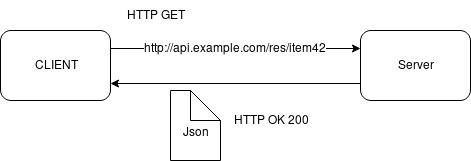
\includegraphics[width=8.5 cm]{Abbildungen/restcommunication.jpg}
	\caption{Schematischer Aufbau WSA via REST}
	\label{fig:rest}
\end{figure}

\begin{itemize}
	\item \textbf{Client-Server:}\\ Der Ansatz der Client-Server Architektur soll verfolgt werden. Durch das Lösen der UI von den Daten der Applikation wird eine Portabilität, Skalierbarkeit und das Vereinfachen der Server-Komponente realisiert, was mittlerweile als Grundlage der kompletten Internet-Architektur gilt, denn der HTTP-Standard selbst beruht auf dieser Architektur.
	\item \textbf{Stateless:}\\ Die Zustandslosigkeit gilt für die Kommunikation zwischen Client und Server. Anfragen des Clients müssen alle Information enthalten um vom Server identifiziert und bearbeitet werden zu können. Einen Zustand oder Session-Informationen liegen somit komplett auf Seiten des Clients.
	\item \textbf{Cache:}\\ Die Antwort auf eine Client-Anfrage kann vom Server als cacheble oder non-cacheble gelabelt werden. Der Cache befindet sich auf der Client-Seite und erlaubt dem Client die Antwort für weitere Anfragen gleicher Art zu verwenden. Dadurch kann teilweise eine Kommunikation zwischen Client und Server unterbunden werden was die Performanz und Effizienz client-seitig stark erhöhen kann.
	\item \textbf{Uniform Interface:}\\ Das Uniform Interface repräsentiert das fundamentale Wesen eines REST-Services. Durch die Uniformierung jeder Ressource werden die Daten von der Architektur gelöst, was eine starke Entkopplung sowie Vereinfachung der Interaktion mit sich bringt. Weiterhin soll jeder Client die nötigen Information und Daten erhalten, die es ihm erlaubt, Ressourcen zu identifizieren und dadurch auch zu modifizieren. Die angefragte Ressource muss nicht die selbe Repräsentation auf Server- und Client-Seite besitzen. Objekte vom Server werden also zum Beispiel via XML oder JSON übertragen, enthalten die definierten Daten, müssen aber nicht dem Datentyp des Server-Objekts entsprechen. Nach Fieldings ist hier das \textit{Hypermedia as the engine of application state (HATEOAS)}-Prinzip mit der wichtigste Faktor. Dieses besagt, dass der Client alle Ressourcen nur über die definierten URI's beziehen kann. Durch diesen Zugang kann der Server dynamisch Daten kommunizieren und weiter verfügbare Adressen der Antwort hinzufügen. Somit wird verhindert, dass der Client fest codierte Information enthalten muss. Dadurch entsteht die Flexibilität des REST-Services.
	\item \textbf{Layered System:}\\ Dem Client muss nicht bekannt sein, ob die Kommunikation direkt mit dem Server stattfindet oder nicht. Die Anfrage wird gestellt und welcher Server aus einem Kollektiv die Antwort sendet, kann nicht zugeordnet werden. Dadurch können Prinzipien wie Load-Balancing und unterschiedliche Web-Sicherheitskriterien realisiert werden. 
	\item \textbf{Code on demand(optional):}\\ Dieser Schritt ist optional und beschreibt die Möglichkeit nach Anfrage ausführbaren Code vom Server zum Client zu transferieren, wie zum Beispiel Skripte in JavaScript. Somit kann der Server zeitweise die Funktionalität der Client-Applikation beeinflussen.
\end{itemize} 
\begin{figure}[ht]\centering
	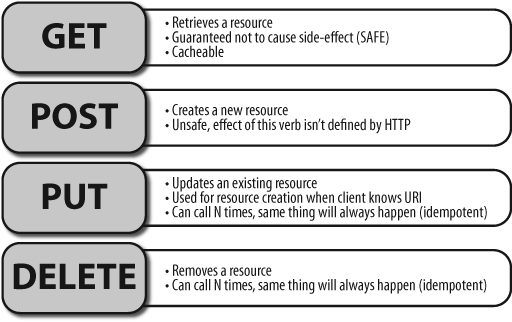
\includegraphics[width=8.5 cm]{Abbildungen/RESTful-operations}
	\caption{Beschreibung der Standard HTTP Methoden in der REST-Architektur. Quelle: http://www.itersdesktop.com/}
	\label{fig:restCalls}
\end{figure}
Im Kontext von Web-Services, welche sich an die REST-Vorgaben binden, wird zumeist die Kommunikation über HTTP umgesetzt. Die API wird über eine Basis-URL angesprochen, über welche dann die benötigten Ressourcen angefragt werden müssen. HTTP bietet eine gewisse Anzahl an Standardmethoden(hauptsächlich: \textit{GET, PUT, POST, DELETE}) die auch für den Datentransfer in einer RESTful-API genutzt werden. Die grundlegenden Eigenschafen der Methoden finden sich im Bild \ref{fig:restCalls}. Diese Methoden repräsentieren auch die bekannten \textit{CRUD}-Operationen(Create, Read, Update, Delete) zur Datenverwaltung und Datenverarbeitung. Eine mögliche Variante mit den entsprechenden HTTP-Befehlen ist in der Tabelle \ref{tab:httptable} zu sehen. Es gilt weiterhin zu erwähnen, dass eine URL mit der entsprechenden HTTP-Methode als eindeutig gilt. Die URL kann jedoch mit einer weiteren HTTP-Methode genutzt werden. Dadurch wird festgelegt welche von den CRUD-Operation auf die entsprechende Ressource angewandt werden darf. 

\begin{table}[hbt]
	\caption{HTTP Methoden für spezifische URL's}
	\centering
	\begin{tabular}{ |p{2cm}|p{5.5cm}|}
		\toprule
		\cmidrule(r){1-2}
		URL & \textbf{http://api.example.com/res/item42}\\
		\midrule
		GET & Eine Repräsentation des Items42 wird an den Client übertragen\\
		\midrule
		POST & Wird zum Erstellen neuer Ressourcen verwendet, würde in diesem Fall eher nicht genutzt werden\\
		\midrule
		PUT & Item42 wird überschrieben oder erstellt wenn noch nicht vorhanden\\
		\midrule
		DELETE & Das adressierte Element Item42 wird gelöscht\\
		\bottomrule
	\end{tabular}\\
	\label{tab:httptable}
\end{table}

\subsection{REST vs. SOAP}
Bevor sich REST im Bereich der verteilten Anwendung etablierte, war die größte Vertreter für die Kommunikation innerhalb einer SOA das SOAP. Bei SOAP handelt es sich um eine RPC Middleware die zum Beispiel HTTP, SMTP oder FTP als Transportprotokoll für XML als Nachrichtenformat verwendet. Schon im grundsätzlichen Ansatz unterscheiden sich beide Herangehensweisen. Wird bei REST von einer exakten Uniformierung jeder Ressource gesprochen, die somit auch immer separat angesprochen werden können, so wird bei SOAP mit einem Dispacher gearbeitet. In sogenannten Envelopes werden alle Anfragen an den Server via XML mit dem HTTP-Post-Befehl an den zentralen Dispatcher geleitet. Die Anfrage gehen an genau eine URL die den Dispatcher adressiert. Im Listing \ref{envelopesoap} ist ein SOAP-Request mit seiner korrespondierenden Response zu sehen. Im Body wird eine \textit{GetStockPrice} Anfrage gestellt für das Unternehmen IBM. Im Body der Antwort wird somit die \textit{GetStockPriceResponse} mit dem Wert von 34,5 übermittelt. Die URL \textit{http://www.example.org/stock} spricht den Dispatcher des Webservers an. Dieser verteilt die Anfrage an die richtige Methode, hier \textit{GetStockPrice}. Diese Methode muss auf dem Server verfügbar sein. Durch die Anfrage wird ein Methodenaufruf mit den gelieferten Parametern durchgeführt. Das Ergebnis des Methodenaufrufs wird als Response in einem neuen Envelope zurück geliefert. Da jede Antwort einer exakten Anfrage gilt, ist ein erneutes stellen der gleichen Anfrage nicht möglich. Somit entfällt eine Möglichkeit caching auf Seiten des Clients zu betreiben.

\begin{lstlisting}[caption=Beispiel: SOAP-Request und SOAP-Response als Envelope, label=envelopesoap, language=xml]
 POST /InStock HTTP/1.1
Host: www.example.org
Content-Type: application/soap+xml; charset=utf-8
Content-Length: nnn

<?xml version="1.0"?>

<soap:Envelope
xmlns:soap="http://www.w3.org/2003/05/soap-envelope/"
soap:encodingStyle="http://www.w3.org/2003/05/soap-encoding">

<soap:Body xmlns:m="http://www.example.org/stock">
<m:GetStockPrice>
<m:StockName>IBM</m:StockName>
</m:GetStockPrice>
</soap:Body>

</soap:Envelope>

--------------------------------------------

 HTTP/1.1 200 OK
Content-Type: application/soap+xml; charset=utf-8
Content-Length: nnn

<?xml version="1.0"?>

<soap:Envelope
xmlns:soap="http://www.w3.org/2003/05/soap-envelope/"
soap:encodingStyle="http://www.w3.org/2003/05/soap-encoding">

<soap:Body xmlns:m="http://www.example.org/stock">
<m:GetStockPriceResponse>
<m:Price>34.5</m:Price>
</m:GetStockPriceResponse>
</soap:Body>

</soap:Envelope>
\end{lstlisting}
Ebenso wie REST wurde SOAP vom W3C spezifiziert. Unterschied ist allerdings, bei REST handelt sich um einen Architekturstil bei SOAP um ein Protokoll. in der Spezifikation steht zum Beispiel, dass ausschließlich XML als Datenformat verwendet wird und was ein XML wohl definiert um als SOAP konform zu gelten \cite{w3cSOAP}. Der Unterschied zu REST liegt hier darin, dass außer XML bei REST weitere Datenformate wie zum Beispiel JSON und YAML verwendet werden können. Die genaue Adressierung der Ressourcen unter REST erlaubt eine leichtgewichtige Transportmöglichkeit. Metadaten, wie das Encoding oder der Content-Type, werden im Header des HTTP-Requests codiert. Zusätzliche Information werden nicht benötigt. SOAP hingegen bietet diese Möglichkeit nicht. Durch die Konvention, welche Bestandteile ein XML-Envelope vorzuweisen hat, ist diese Leichtigkeit nicht zu erreichen. Das XML-Dokument muss auf Seiten des Sender aufgebaut und anschließen validiert werden um die Konformität zu bewahren. Dadurch werden zusätzliche Metadaten zur Beschreibung der Datei dem XML-Dokument hinzugefügt. Gerade bei einfachen Anfrage, zum Beispiel eine Zustandsabfrage wahr oder falsch, ist das Verhältnis von Nutz- zu Metadaten eher mäßig. Je aufwändiger die Anfrage desto besser entwickelt sich das Nutzlastenverhältnis. Anfragen eine XML-Dokuments werden immer atomar ausgeführt. Somit können komplexe Sachverhalte in einer Anfrage definiert werden und sequentiell abgearbeitet werden. Bei REST werden meist leichtgewichtige Schnittstellen exponiert die genau eine Anfrage nach einer bestimmten Ressource beantworten. Somit sind bei komplexeren Schritten mehre Anfragen nötig. Dadurch ist der Kommunikationsaufwand etwas höher als bei SOAP. Relativ ähnlich verhalten sich die beiden in Bezug auf die Interaktion. Da beide Plattform unabhängige Datenformate verwenden entfaltet sich ein großen Potenzial in der Nutzung. Programme jeglicher Art, entwickelt in einer belieben Programmiersprache, welche die Datenformate ebenso unterstützen, können mit den Schnittstellen interagieren. Bei REST muss eine API-Beschreibung mit den exponierten URL's, bei SOAP die URL mit den möglichen Methodenaufrufen öffentlich gemacht werden. Bei SOAP wird die Beschreibung meist als WSDL(\textit{Web Services Description Language}) \cite{w3cWSDL} vorgelegt. In dem WSDL-File werden alle Funktionen, Daten und Datentypen beschrieben. Es werden im wesentlichen die Operation definiert, die von außen zugänglich sind. Mit diesem WSDL-File wird auch die Validierung des XML-Dokuments durchgeführt. Es handelt sich auch hierbei um einen weiteren Standard definiert vom W3C.
\subsection{Evaluierung}
Durch die Kriterien welche Fieldings vorgibt, sowie durch den Vergleich mit SOAP haben sich einige Punkte heraus kristallisiert, welche hier nochmals kurz zusammen gefasst werden. \\ REST wird als leichte Schnittstelle definiert, in welcher jede URL eine exakte Ressource anspricht. Die Kommunikation findet über HTTP mit den üblichen HTTP-Methoden statt. Dem Client ist nicht bekannt mit welchem Server genau die Kommunikation stattfindet, was eine hohe Flexibilität und Skalierbarkeit generiert. Es müssen für alle benötigten Informationen immer die entsprechenden Requests angefragt werden, was wiederum zu einem starken Kommunikationsbedürfnis zwischen Client und Server führt. Durch caching auf der Client-Seite kann dem etwas vorgebeugt werden. Meta-Informationen werden innerhalb des HTTP-Headers gespeichert und im Body befinden sich nur die Nutzdaten. Dadurch entsteht ein hohes Nutzlastverhältnis. Die Information des Bodys kann in unterschiedlichen Datenformaten verschickt werden, was eine vielfältige Anwendungsmöglichkeit bietet. \\ Durch die vielen Vorteile ist leicht nachzuvollziehen wieso REST aktuell der vorherrschende Architektur Stil in Sachen Web-Anwendung ist. Im Bereich von großen Enterprise-Lösungen bis hin zu kleinen leichten Web-Anwendungen werden Applikationen nach dem REST-Architekturstil realisiert. 

\section{Entwicklungsansatz und Aufbau}
Um zu Verstehen wie sich eine solche RESTful API zusammen setzt, wird in folgendem die grundlegende Spezifikation \textit{JAX-RS 2.0 - Java API for RESTful Web Services} vorgestellt. Anschließend wird ein in Java realisiertes Beispiel geschildert um die einzelnen Komponenten zu analysieren. 

\subsection{JAX-RS - die Basis für REST-Services in Java}
Bei JAX-RS handelt es sich um die Java eigene Programmierschnittstelle um das Entwickeln von Webservices unter Verwendung des Architekturstils REST zu vereinheitlichen. Die API wurde, bestehend aus einem Konsortium(u.a. Red Hat, Oracle, Fujitsu, Motorola) unter der Führung von Oracle/Sun Microsystems, entwickelt und spezifiziert. Die eigentliche Spezifikation \cite{jaxrs1.1} stammt aus dem Jahre 2009 und wird unter dem Java Specification Request \cite{spezreq} 311 geführt. Es wurden jedoch nicht alle Funktionalitäten in der Version 1 beziehungsweise 1.1 spezifiziert, was zur Folge hatte, dass am Januar 2011 eine Arbeitsgruppe zur Entwicklung von JAX-RS 2.0 gegründet wurde. Die wichtigste Neuerung war das Realisieren des \textit{HATEOAS}-Prinzips. JAX-RS ist seit Java EE 6 Teil der Plattform. In Java SE sind die Schnittstellen standardmäßig nicht vorhanden und müssen separat als Abhängigkeiten geladen werden. Die Beschreibung des JSR 339 für JAX-RS 2.0 \cite{spezJSR339} beinhaltet noch viele weitere Informationen. Da es sich bei JAX-RS um eine vollwertige Spezifikation einer Schnittstelle handelt fällt diese relativ groß aus. Da jedoch zum Programmieren des Beispiels ein Framework verwendet wird, wird auf eine detaillierte Beschreibung der Spezifikation verzichtet. Nachgelesen werden kann die Spezifikation in Quelle \cite{jaxrs1.1}. Ebenso wird Jersey \cite{jersey} als Referenzimplementierung genannt. Sie stellt das Basis-Framework für die beiden JAX-RS API's. Um die meisten spezifizierten Eigenschaften dieser Java-API zu verwenden wie heutzutage üblich auf Annotationen zurück gegriffen. Sie vereinfachen das Entwickeln und die Übersicht und sind Hauptinitiator um Clients und Server REST-konform zu gestalten. Im folgenden Beispiel wird eine Applikation mit der schon erwähnten Implementierung Jersey 2.0 umgesetzt. Es gibt natürlich viele weitere Frameworks, wie zum Beispiel JBoss oder Spring. jedoch ist zur Veranschaulichung das Leichtgewicht Jersey ausreichend.
\begin{figure}[ht]\centering
	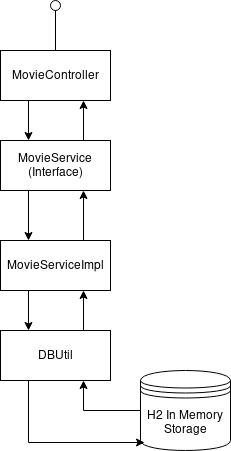
\includegraphics[width=6 cm]{Abbildungen/overview.jpg}
	\caption{Schematischer Überblick zur Movie-Portfolio Applikation}
	\label{fig:overview}
\end{figure}
\subsection{Beschreibung der Beispielapplikation}
Das Szenario in welcher die Applikation genutzt werden soll lautet wie folgt: Ein Nutzer möchte sich sein eigenen Film-Portfolio anlegen. Er würde die Funktion gerne von seinem Rechner aber auch von seinem Smartphone aus benutzen können. Er möchte sich alle Filme die in seiner Liste sind anzeigen lassen, nach einem bestimmten Eintrag suchen, einen Eintrag hinzufügen oder einen Eintrag löschen. Beschrieben wird nun die auf dem Applikations-Server vorhandene Implementierung. \\ Das Projekt ist als Maven-Projekt umgesetzt und nutzt eine Version von Java SE. Alle Jersey-Abhängigkeiten sind somit in der \textit{pom.xml} definiert. Zusätzliche Abhängigkeiten sind \textit{Jackson} und \textit{Gson} zum mapping von Java-Objekten zum Json-Datenformat. Als Datenbankabhängigkeit wird die H2 InMemory-Datenbank verwendet. Da es sich nur um ein Beispiel handelt wurde kein eigenständiger Applikationsserver wie zum Beispiel Tomcat aufgesetzt. Stattdessen wurde auf die eigens dafür mitgebrachte JdkHttpServerFactory von Jersey zurückgegriffen. Diese erstellt zur Laufzeit einen entsprechenden HTTP-Server, sodass auch die Kommunikation via REST stattfinden kann. Die verwendete \textit{pom.xml} findet sich im Anhang in Listing \ref{pom.xml}.
Ein Überblick über den Aufbau der Applikation findet sich in Abbildung \ref{fig:overview}.
\subsection{Serverseite Beispielimplementierung}
Im eben erwähnten Überblick lassen sich einige Information ableiten. Die Applikation exponiert eine Schnittstelle. Über diese kann Informationsaustausch in beide Richtungen stattfinden. Ebenso lässt sich erkennen, dass der \textit{MovieSerivce} als Interface abgebildet ist und die eigentliche Implementierung nachgelagert realisiert wird. In dem Schemata wird das Erstellen des vorab erwähnten HTTP-Servers nicht abgebildet. Da der eingebettete Server von Jersey verwendet wird, fällt die Konfiguration ziemlich gering aus. Die Initialisierung wird in der \textit{MainClass} beim starten der Anwendung direkt mit ausgeführt(vgl. Listing \ref{mainclass.java}). Als Ressourcenkonfiguration wird die MovieResource-Klasse angegeben. Diese enthält die Pfade und Methoden die vom HTTP-Server initialisiert werden sollen, sodass Aufrufe dementsprechend geroutet werden können. Die einzelnen Bestandteile werden in Folgendem im Detail beschrieben.
\lstinputlisting[language=Java, label=mainclass.java, caption={MainClass: Startklasse der Applikation. Startet HTTP-Server und initialisiert die benötigten REST Resourcen}, emptylines=0, flexiblecolumns=false, firstline=10]{../code/RestExample/src/main/java/MainClass.java}
\subsubsection{MovieResource}
Die MovieResource, auch REST-Controller genannt, spiegelt die Schnittstelle programmatisch wider. Für alle Funktionalitäten werden hier die Pfade und die entsprechenden HTTP-Methoden festgelegt. Annotationen wie \textit{@GET} oder \textit{@POST} geben den zu verwendenden HTTP-Aufruf vor. Der Pfad setzt sich aus der Server-URL wie in Listing \ref{mainclass.java} zu sehen, ebenso aus den \textit{@Path}-Annotationen an der Controller-Klasse sowie den entsprechenden Methoden zusammen. In Listing \ref{controller.java} sind diese Annotationen zu sehen. Um den Controller anzusprechen lautet der Pfad \textbf{http://localhost:8080/rest/movies}. Bei der ersten gelisteten \textit{GET}-Methode ist keine Erweiterung des Pfades nötig. Somit führt ein HTTP-GET auf \textit{http://localhost:8080/rest/movies} dazu, dass eine Anfrage nach allen in der Datenbank befindlichen Filmen gestellt wird. Die zweite Methode trägt die Erweiterung \textit{"movieId"}. Hierbei handelt es sich im einen in der URL codierten Parameter.  Somit liefert ein HTTP-GET auf \textit{http://localhost:8080/rest/movies/2} den Film mit der ID 2 aus der Datenbank, wie auch in Abbildung \ref{fig:responsebrowser} zu sehen, beziehungsweise \textit{null} wenn ein Film mit dieser ID nicht vorhanden wäre. 
\begin{figure}[ht]\centering
	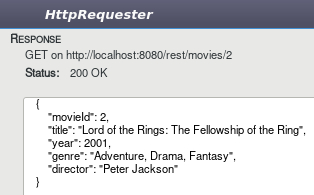
\includegraphics[width=8.5 cm]{Abbildungen/getid2.jpg}
	\caption{Response zum GET-Request auf http://localhost:8080/rest/movies/2}
	\label{fig:responsebrowser}
\end{figure}
\lstinputlisting[language=Java, label=controller.java, caption={Ausschnitt aus der MovieController-Klasse}, emptylines=0, flexiblecolumns=false, firstline=8, lastline=31]{../code/RestExample/src/main/java/MovieResource.java}
Als Rückgabewert wird in beiden Fällen eine HTTP-Response geliefert. Diese enthält bei einem GET-Request laut dem Standard(vgl .\cite{httpcodes}) den HTTP-Code \textit{200 OK}. Im Body werden die Objekte als Json geliefert. Die Annotation \textit{@Produces} besagt, dass Json als Datenformat verwendet werden soll. Das Gson-Objekt ermöglicht es Java-Objekte in das entsprechende Json-Format zu bringen. Ohne die korrekte Formatierung wäre eine Serialisierung der Objekte nicht möglich und es würde zu Fehlern in der Übertragung kommen. Die Definition der weiteren Methoden können im vollständigen Code des MovieController in Listing \ref{moviecontroller.java} gefunden werden. \\ Somit gilt der Controller nur als Berührungspunkt mit der Außenwelt. Die Funktionalität wird durch den darunter liegenden Service realisiert.
\subsubsection{MovieService-Interface}
Der MovieService selbst wurde in diesem Beispiel als Interface implementiert. Durch diese Instanz zwischen Controller und Service-Implementierung wird eine gewissen Stabilität gegenüber dem Controller gewährleistet jedoch kann man die verwendete Implementierung beliebig austauschen sofern die im Interface festgelegten Methoden überschrieben werden. Dadurch ergibt sich eine Flexibilität gegenüber der Service-Implementierung. 
\lstinputlisting[language=Java, label=serviceinterface.java, caption={MovieService Interface des Movie-Portfolios}, emptylines=0, flexiblecolumns=false, firstline=2]{../code/RestExample/src/main/java/MovieService.java}
In Listing \ref{serviceinterface.java} sind die gewünschten Funktionalitäten abgebildet. Wie es für jede spezielle Anfrage eine exakte URL gibt, wird auch jede Funktionalität mit einer eigenen Implementierung abgedeckt.
\subsubsection{MovieService-Implementierung}
Hierbei handelt es sich um die konkrete Implementierung der dem Interface zugrunde liegenden Funktionen. Da diese Beispielanwendung sehr klein gehalten ist, ist die einzige Aufgabe das Lesen und Schreiben der Datenbank. Hierzu wird nur die entsprechende Datenbank-Instanz benötigt. Der Programm-Code findet sich in Listing \ref{serviceimpl.java}.
\lstinputlisting[language=Java, label=serviceimpl.java, caption={MovieService Implementierung des Movie-Portfolios}, emptylines=0, flexiblecolumns=false]{../code/RestExample/src/main/java/MovieServiceImpl.java}
\subsubsection{DBUtil}
Wie der Name schon verlauten lässt, handelt es sich hierbei um eine Hilfsklasse. Da keine konkrete Datenbank verwendet wird, ebenso wenig DAO-Klassen, werden die Lese- und Schreibvorgänge in einer Datenbank im Speicher des Rechners durchgeführt. Diese wird mit dem Anlegen einer DBUtil-Instanz angelegt und wird mit Beendigung des Programms zerstört. Um die Applikation funktionstüchtig zu implementieren wurde eine Art von Datenspeicher benötigt. Jedoch handelt es sich hierbei nicht unbedingt um einen relevanten Teil des REST Architekturstils. Die essenziellen Bestandteile können im Listing \ref{dbutil.java} im Anhang betrachtet werden.
\subsection{Clientseite Beispielimplementierung}
Grundlegend ist die Realisierung der REST-API durch die Implementierung der Server-Seite abgeschlossen. Eine Benutzung kann über den Browser, Kommandozeilenbefehle wie \textit{curl} oder allen weiteren Programmen, welche es ermöglichen HTTP-Request zu verschicken, stattfinden. Ebenso besteht natürlich die Möglichkeit eine Java-Client programmatisch darzustellen, um innerhalb einer Applikation mit der REST-API zu interagieren. Auch hier bietet das Jersey-Framework wieder die nötigen Bordmittel. Beispielhaft kann eine Client-seitige GET-Anfrage nach einem besagten Film aus unserem Portfolio wie in Listing \ref{restclient} aufgebaut sein.
\begin{lstlisting}[caption=Beispiel: Beispielhafte Java-Client Anfrage, label=restclient, language=java, emptylines=0, flexiblecolumns=false]
...
private List<Movie> getMoviesResponse() {
try {

Client client = Client.create();
WebResource webResource = client.resource("http://localhost:8080/rest/movies");
ClientResponse response = webResource.accept("application/json").get(ClientResponse.class);
if (response2.getStatus() != 200) {
throw new RuntimeException("Failed : HTTP error code : " + response.getStatus());
}

List<Movie> output = response.getEntity(new GenericType<List<Movie>>(){});


} catch (Exception e) {
e.printStackTrace();
}
}
...
\end{lstlisting}
Die Klassen Client, WebResource sowie ClientResponse werden alle durch das Jersey-Framework zur Verfügung gestellt. Der Client bekommt die URL für die geforderte Ressource, hier die Liste aller Filme. Durch das tragen der URL wird der Client zur WebResource. Diese bietet die Möglichkeit die entsprechenden Requests zu stellen. Als Antwort wird ausschließlich Json akzeptiert und mit dem folgenden Methodenaufruf \textit{get(ClientResponse.class)} wird der HTTP-Request ausgeführt. Die ClientResponse-Klasse birgt die komplette Antwort, also HTTP-Header und Body. Somit können wie im Beispiel der HTTP-Status auf Richtigkeit geprüft werden bevor die Daten des Bodies verarbeitet werden. Der GenericType wird bei zum Beispiel bei allen Arten von Collections verwendet. Somit wird das erhaltene Json in die benötigte Java-Objekt Konstellation gebracht, hier eine Liste mit den Filmen. Dieser Zusatz ist beim Übertragen einfacher Daten oder einzelner Objekte nicht notwendig. Zu erwähnen ist weiterhin, dass der verwendete Datentyp Movie im Client nicht dem Datentyp vom Server entsprechen muss. Es müssen nicht alle Felder vorhanden sein, ebenso wenig ist der Datentyp auf nur die übertragenen Felder beschränkt. Dies bestätigt auch die \textit{Uniform Interface} Richtlinie von Fielding. Jedoch muss der Bezeichner des Objekt-Attributs den Namen des JSON-Attributs tragen.

\section{Zusammenfassung}
Beschrieben wurde der REST Architekturstil. Es wurden grundlegenden Eigenschaften nach Fielding erläutert welche ein diese Architekturart mit sich bringen muss um auch als solche bezeichnet und genutzt zu werden. Mit diesen sechs Eigenschaften wurden nicht nur der Großteil der heute existierenden Web-Anwendungen sondern auch das HTTP selbst entwickelt. Es existieren viele Frameworks die es sich zur Aufgabe gemacht haben die JAX-RS API von Java weiter zu entwickeln und die Benutzung zu vereinfachen und zu erweitern. Anhand des Referenz-Frameworks Jersey 2.0 wurde eine beispielhafte Implementierung einer RESTful-API durchgeführt. Nochmals herauszustellen ist die Einfachheit mit welcher solch eine Schnittstelle realisiert werden kann. Hauptsächlich mit Annotationen und den gelieferten Klassen gelingt die Implementierung schnell und effektiv. Ebenso ist deutlich zu erkennen, dass der Aufbau einfach gehalten und leicht nachvollziehbar ist. Es wurden im Film-Portfolio Beispiel nicht alle Aspekte speziell beleuchtet, jedoch sind die essenziellen Notwendigkeiten, wenn auch nicht mit allen Voraussetzungen, wie die Umsetzung des \textit{Uniform Interfaces} dargestellt. Alles in Allem wird klar wieso sich REST an vorderster Front zur Realisierung von \textit{Web Services Architectures} befindet. Flexibilität, einfache Umsetzung sowie Skalierbarkeit sind nur einige Vorteile die REST für die Kommunikation zwischen Applikationen im WWW mit sich bringt. Diese breite Funktionalität bereitet den Weg für ein verteiltes Entwickeln von Anwendungen ebenso wie ein einfachen Anbinden von freien oder kommerziellen Diensten anderer Anbieter.
\begin{figure}[ht]\centering
	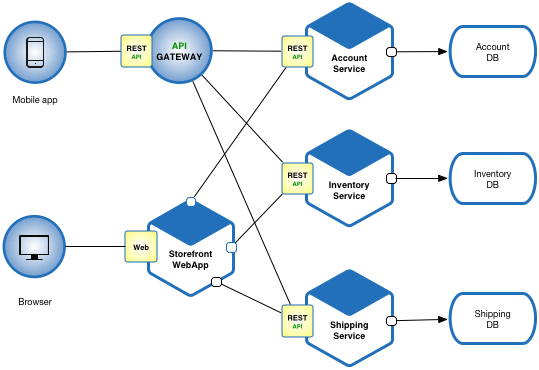
\includegraphics[width=8.5 cm]{Abbildungen/Microservice_Architecture.png}
	\caption{Aufbau einer Microservice-Architektur}
	\label{fig:micro}
\end{figure}
\subsection{Ausblick}
Gerade das Nutzen schon vorhandener Dienste birgt ein interessantes Thema. Die Mircoservice-Architektur. Im Zuge dieser wird es sich zum Ziel gemacht, eigenständige Komponenten als unabhängige Services zu implementieren und zu deployen. Somit sollen viele einzelne Dienste entstehen die wiederum in unterschiedlichen Projekten und Applikationen genutzt werden können. Der Datenaustausch findet auch zwischen den einzelnen Services mit REST statt und um die Nutzung eines solchen Dienstes zu beanspruchen muss über die exponierte API kommuniziert werden. Einen kurzen Überblick gibt die Grafik \ref{fig:micro}.
Viele grundlegende Informationen über den Aufbau einer Microservice-Architektur findet man in Quelle \cite{microservice}. 

\clearpage
\appendix
\cleardoublepage
\onecolumn
\newpage
%----------------------------------------------------------------------------------------
%	REFERENCE LIST
%----------------------------------------------------------------------------------------

\bibliographystyle{unsrt}
\bibliography{Literatur}

%----------------------------------------------------------------------------------------

\clearpage
\appendix
\cleardoublepage
\newpage
\onecolumn

\section{Listings}
\lstinputlisting[language=XML, label=pom.xml, caption={POM.xml der Beispielanwendung}, emptylines=0, flexiblecolumns=false]{../code/RestExample/pom.xml}
\newpage
\lstinputlisting[language=JAVA, label=moviecontroller.java, caption={Vollständiger Code des MovieControllers}, emptylines=0, flexiblecolumns=false]{../code/RestExample/src/main/java/MovieResource.java}
\newpage
\lstinputlisting[language=JAVA, label=dbutil.java, caption={Auszüge aus der DBUtil Klasse}, emptylines=0, flexiblecolumns=false, linerange={10-36, 47-70, 212-212}]{../code/RestExample/src/main/java/DBUtil.java}
\newpage
\end{document}